
\documentclass[]{article}% insert '[draft]' option to show overfull boxes

\usepackage{color}
\usepackage{graphicx,psfrag}
\usepackage{subfigure}
\usepackage{epstopdf}
\usepackage{float}


\usepackage{amssymb}
\usepackage{amsmath}
\usepackage{epstopdf}
\usepackage{morefloats}

\usepackage{graphicx}
\usepackage{amssymb}
\usepackage{appendix}
\usepackage{listings}

%\usepackage{xcolor}
\usepackage{framed}


\lstset{language=c,morecomment=[l]{//} , label=DescriptiveLabel}
\lstset{frame=shadowbox,}
\lstset{caption=\lstname }


\textwidth = 6.5 in \textheight = 9 in \oddsidemargin = 0.0 in
\evensidemargin = 0.0 in \topmargin = 0.0 in \headheight = 0.0 in
\headsep = 0.0 in
\parskip = 0.2in
\parindent = 0.25in

%\newcommand{\comment}[1]{}

%\newtheorem{theorem}{Theorem}
%\newtheorem{corollary}[theorem]{Corollary}
%\newtheorem{definition}{Definition}
%\usepackage{epstopdf
\newcommand{\pd}[2] {\frac{\partial #1}{\partial #2}}
\newcommand{\gfilter}[1] {\overline{#1}}
\newcommand{\tfilter}[1] {\widehat{#1}}
\newcommand{\average}[1] {\langle{#1}\rangle}
\newcommand{\absolute}[1] {\left|{#1}\right|}
\newcommand{\favre}[1] {\widetilde{#1}}

\title{HPC Project: Shade Model Optimization}

\author{Troy Axthelm, Jared Baker, Matthew J. Brazell, Nels Frazier}

\begin{document}

\maketitle
\begin{figure}[H]
\centering
  \begin{tabular}{@{}cccc@{}}
    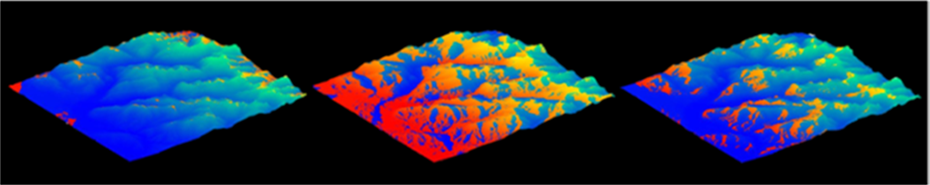
\includegraphics[width=.75\textwidth]{./figures/titleBar.png} 
  \end{tabular}
  \caption{}
  \label{}
\end{figure}

%--------------------------------------------------------------------------------------------------------------------------------------

\listoffigures



\section{Introduction}

%Talk about the purpose, creaters, and users....

This program is designed to model shade given elevation and location information for a selected land area. With this information a model of watershed can be created for primary use by CI-Water Project for predicting locations for forest fire remediation. The uploaded land area of interest can simply be downloaded off of GIS, the user can select a time interval over the course of a specific day of the year. The GPS coordinates of the land area as well as day of the year provide solar angle along with the topography of the land indicate if an area is shaded or not. Currently the program  only indicates if an element of the land area is shaded or not shaded. No information of temperature or partial shading is provided and may be a future goal however currently this information alone is sufficient for CI-Water Project's needs.

The original program was created by Troy Axthelm and Jingyu Li  funded by CI-Water Project. For more information and location of the open source code please see the link below:

https://sites.google.com/site/uwyoshademodel/

As a project for a graduate coarse: Designing and Building Applications for Extreme Scale Systems lead by instructor William Gropp and Professor Craig Douglas, our group intends make improvements in performance leading to faster simulations as well as making the program more flexible and easier to use for the user during runtime as well as post processing and visualization.

\subsection{Initial Benchmarking}
\subsubsection{Parlib MPI}

For performance just using MPI instead of Parlib removes a level of Libraries as well as making threading too abstract????.

\subsubsection{MPI}

\subsection{Coding Improvements}
\subsubsection{Algorithmic Improvements}
introduce global constants
reduce built in algebraic functions
example code from landReader.c:

$temp.latitude = latitude*180.0/(4*atan(1))$;	$//convert the latitude to degrees	$

where $4*atan(1) = 3.141592653589793 = \pi$

\subsubsection{Linear Memory}


\subsubsection{Improvements for User}
Add input file to modify time intervals and....

output file structure



\subsection{Results}
\subsubsection{Final BenchMark}

\subsection{Conclusion}


%\begin{table}[ht]
%\caption{Threading Copy Results}
%\centering
%\begin{tabular}{c c c}
%\hline\hline
% Nt & Time for Loop(s) & Rate [MB/s]\\ [0.5ex] 
%\hline
%1 & 5.352E-04 & 5979\\ 
%2 & 1.058E-03 & 3024\\
%4 &  2.715E-03 & 1178\\
%6 & 7.943E-03 & 402 \\
%8 & 1.479E-02 & 216 \\
%[1ex]
%\hline
%\end{tabular}
%\label{table:norm_high}
%\end{table} 

%----------------------------------------------------------------------------------------------------------------------------------------------------------------



%----------------------------------------------------------------------------------------------------------------------------------------------------------------

\newpage
\appendix
\section{\\Original Code} \label{App:AppendixA}

\lstinputlisting{./orig_code/main.c}
\lstinputlisting{./orig_code/azimuth.c}
\lstinputlisting{./orig_code/hourAngleTest.c}
\lstinputlisting{./orig_code/landReader.c}
\lstinputlisting{./orig_code/localHourAngle.c}
\lstinputlisting{./orig_code/parlib_mpi.c}
\lstinputlisting{./orig_code/parlib.c}
\lstinputlisting{./orig_code/solarAltitude.c}
\lstinputlisting{./orig_code/solarAltTest.c}
\lstinputlisting{./orig_code/sunDeclination.c}
\lstinputlisting{./orig_code/test.c}
\lstinputlisting{./orig_code/tilt.c}
\lstinputlisting{./orig_code/timeDifference.c}


%----------------------------------------------------------------------------------------------------------------------------------------------------------------

%\newpage
%\appendix
%\section{\\Code} \label{App:AppendixA}
%
%\begin{verbatim}
%
%\end{verbatim}



\end{document}

